\documentclass[14pt, fleqn, xcolor={dvipsnames, table}]{beamer}
\usepackage[T2A]{fontenc}
\usepackage[utf8]{inputenc}
\usepackage[english,russian]{babel}
\usepackage{amssymb,amsfonts,amsmath,mathtext}
\usepackage{cite,enumerate,float,indentfirst}
\usepackage{cancel}
\usepackage{graphicx}
\usepackage{animate}

\usepackage{tikz}
% \usepackage{enumitem}
\usetikzlibrary{shadows}

% \usepackage{enumitem}
% \setitemize{label=\usebeamerfont*{itemize item}%
%   \usebeamercolor[fg]{itemize item}
%   \usebeamertemplate{itemize item}}

\graphicspath{{images/}}

\usetheme{Madrid}
\usecolortheme{seahorse}
\renewcommand{\CancelColor}{\color{red}}

\setbeamercolor{footline}{fg=Blue!50}
\setbeamertemplate{footline}{
  \leavevmode%
  \hbox{%
  \begin{beamercolorbox}[wd=.333333\paperwidth,ht=2.25ex,dp=1ex,center]{}%
    И. Кураленок, Н. Поваров, Яндекс
  \end{beamercolorbox}%
  \begin{beamercolorbox}[wd=.333333\paperwidth,ht=2.25ex,dp=1ex,center]{}%
    Санкт-Петербург, 2014
  \end{beamercolorbox}%
  \begin{beamercolorbox}[wd=.333333\paperwidth,ht=2.25ex,dp=1ex,right]{}%
  Стр. \insertframenumber{} из \inserttotalframenumber \hspace*{2ex}
  \end{beamercolorbox}}%
  \vskip0pt%
}
\newcommand\indentdisplays[1]{%
     \everydisplay{\addtolength\displayindent{#1}%
     \addtolength\displaywidth{-#1}}}
\newcommand{\itemi}{\item[\checkmark]}

\newenvironment{mydescription}[1]
  {\begin{list}{}%
   {\renewcommand\makelabel[1]{\color{blue}##1:\hfill}%
   \settowidth\labelwidth{\makelabel{#1}}%
   \setlength\leftmargin{\labelwidth}
   \addtolength\leftmargin{\labelsep}}}
  {\end{list}}

\title{Уменшение размерности: SOM\\\small{}}
\author[]{\small{%
И.~Куралёнок,
Н.~Поваров}}
\date{}
\begin{document}

\begin{frame}
\maketitle
\small
\begin{center}
\vspace{-60pt}
\normalsize {\color{red}Я}ндекс \\
\vspace{80pt}
\footnotesize СПб, 2014
\end{center}
\end{frame}
\section{SOM}

\begin{frame}{SOM}{Самоорганизующиеся сети Кохоненна}
\textbf{Идея:} отобразить многомерное пространство в граф, зафиксированной структуры так, чтобы как можно лучше сохранить взаимные расстояния. \\
\textbf{Графы бывают разные:}
\begin{itemize}
  \item Простая 2/3-х мерная сеть
  \item Шестигранная сетка
  \item Односвязная “нить”.
\end{itemize}
\end{frame}

\begin{frame}{SOM}{процесс обучения}
Можно представить так: кидаем платок и расправляем его.
\begin{center}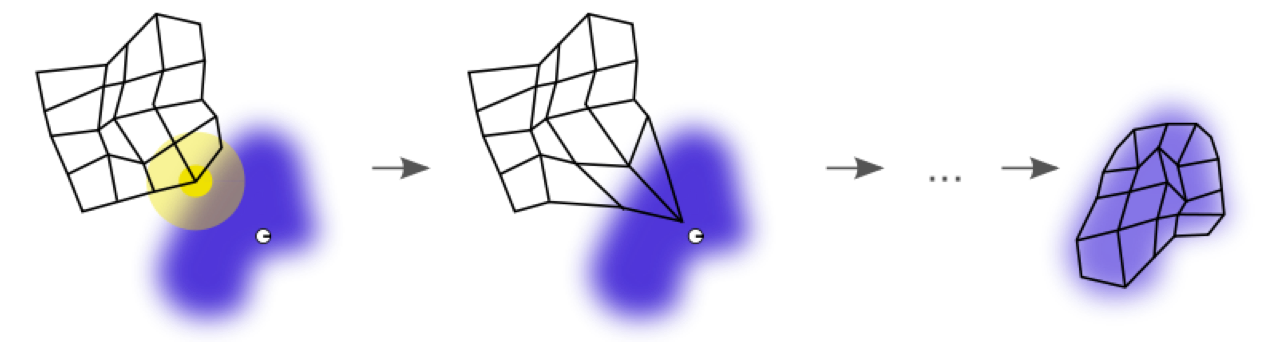
\includegraphics[width=0.7\textwidth]{SOM.png}\end{center}
\end{frame}

\begin{frame}{SOM}{алгоритм}
\textbf{Дано:} функция расстояния по графу ($G$), множество точек ($X \in \mathbb{R}^n$), дискаунт за расстояние ($q$), дискаунт за итерацию ($s$) 
\begin{enumerate}
  \item Инициализируем точки, соответствующие узлам графа $g_i$ в $\mathbb{R}^n$
  \item Выберем случайную точку $x^t$ в $X$
  \item Находим ближайший $g_{i_0}$
  \item ``Двигаем'' $g_i$ в сторону точки $x^t$, по принципу ``чем дальше, тем меньше'':
  $$
    g_i^{t+1} = g_i^t + q(G(i, i_0), t)s(t)(x_t - g_t)
  $$
  \item Переходим в п.2 пока не сошлось.
\end{enumerate}
\end{frame}

\begin{frame}{SOM}{свойства}
Что можно с их помощью делать:
\begin{itemize}
  \item Смотреть на данные ``глазами''
  \item Если из области следует какая-то структура, то можно подобрать ее распределение таким образом
  \item Аля PCA по 1D кривулинам, полученным с помощью SOM
\end{itemize}
Проблемы:
\begin{itemize}
  \item Результат существенно зависит от подбора начальных $g_i \Rightarrow$ зачастую не воспроизводим
  \item Никаких гарантий сходимости при $s(t) = 1$
  \item Никаких хороших математических свойств.
\end{itemize}
Но, it just works!
\end{frame}

\begin{frame}{SOM}{рекомендации SOMоводов}
\begin{itemize}
  \item Выбирать начальные значения не по рандому, а по PCA2
  \item Выбросить выбросы/сгладить движение от дистанции
  \item Бегать не в одном и том же порядке по множеству
  \item По минимуму использовать $s$.
\end{itemize}
\end{frame}

\section{Кластерный анализ}

\begin{frame}{Кластерный анализ}{определение}
{\color{blue}Определение (Wikipedia)} \\
\italic
\textbf{Кластерный анализ (англ. cluster analysis): }задача разбиения заданной выборки объектов (ситуаций) на подмножества, называемые кластерами, так, чтобы каждый кластер состоял из схожих объектов, а объекты разных кластеров существенно отличались.
\end{frame}

\begin{frame}{Кластерный анализ}{виды}
\begin{itemize}
  \item Иерархические методы (connectivity-based)
  \item Основанные на центройдах
  \item Генеративные модели (distribution-based)
  \item Ограниченные (constraint-based).
\end{itemize}
\end{frame}

\begin{frame}{Кластерный анализ}{иерархические методы}
\small
\textbf{Цель:}
$$
  C: \forall c \in X, c \in C_i, \exists c^* \in C_i : d(c, c^*) < \epsilon
$$
\textbf{Алгоритм (однсвязный):}
\begin{enumerate}
  \item Выбираем случайную точку $x$ и кладём её $C_i$
  \item Ищем соседей $x$ ближе, чем $\epsilon$ и добавляем их в $C_i$
  \item Если соседи $x$ кончились, берём следующую точку из $C_i$ и проделываем п. 2
  \item Замкнув $C_i, i = i+1$ и переходим к п. 1
\end{enumerate}
\textbf{Замечания:} можно сделать более, чем односвязное замыкание, так как подобных делений много, результат сильно зависит от рандома, сложность $O(n^3)$.
\end{frame}

\begin{frame}{Кластерный анализ}{иерархические методы, плотность}
\small
\textbf{Цель:}
$$
  C: \forall c \in X, \exists C^* \subseteq C_i: |C^*| > m, \forall c \in C^* d(c, c^*) < \epsilon
$$
\textbf{Алгоритм (DBSCAN):}
\begin{enumerate}
  \item Выбираем случайную точку $x$ и кладём её $S$
  \item Для каждой точки из $S$:
  \begin{enumerate}
    \item Ищем соседей в радиусе $\epsilon$
    \item Если точка ещё не в каком-либо кластере, кладём точки в $C_i$
    \item Если таких соседей больше $m \in C_i$, то добавляем всех соседей в $S$. 
  \end{enumerate}
  
\end{enumerate}
\textbf{Замечания:} сложность $O(n^2)$, повязаны на поиск ближайших соседей.
\end{frame}

\begin{frame}{Кластерный анализ}{центроиды}
\small
\textbf{Цель:}
$$\begin{array}{l}
  \overline{x}_c = \frac{1}{|c|}\sum_{x \in C} x \\
  min_C \sum_{c \in C, |C| = k} \sum_{x \in c} \|x - \overline{x}_c\|
\end{array}$$
Такая задача NP-полная. \\
\textbf{Приблизительный алгоритм (k-means/Lloyd's):} \\
{\color{blue}инициализация:} выберем $k$ штук $\overline{x}_c$; \\
{\color{blue}assignement step:} для каждой точки $x \in X$ ищем ближайший $\overline{x}_c$ и относим её к соответствующему кластеру $c$; \\
{\color{blue}update step:} пересчитываем $\overline{x}_c$, переходим к assignement step, пока не сойдётся; \\
\end{frame}

\begin{frame}{Кластерный анализ}{k-means, свойства}
\begin{itemize}
  \item Никаких гарантий сходимости для k-means
  \item Сильная зависимость от начальных параметров
  \item Вместо центройдов можно использовать медианы
  \item Один из самых простых случаев EM $\Rightarrow$ можно попробовать EM гауссовой смеси напрямую.
\end{itemize}
\end{frame}


\begin{frame}{Кластерный анализ}{центройды, FOREL}
\begin{enumerate}
  \item Выбираем случайную точку $x$, зовём её ``центром тяжести'' $R$
  \item Добавляем все точки из $\epsilon$-окрестности $R$ в $C_i$
  \item Пересчитываем $R = \argmin_{x_0 \in C_i}\sum_{x\in C_i} \|x - x_0\|$.
\end{enumerate}
\textbf{Свойства:} 
\begin{itemize}
  \item Быстрый и тупой
  \item Не сходится
  \item Результат опять зависит от рандома.
\end{itemize}
\end{frame}

\begin{frame}{Кластерный анализ}{центройды, quality threshold}
\footnotesize
\begin{enumerate}
  \item Для каждой точки строим $\epsilon$-окрестности
  \item Сортируем полученные множества по уменьшению мощности
  \item Объявляем первое множество в списке кластером, если количество элементов в нем $> N$, иначе выходим
  \item Отсеиваем из окрестностей содержание нового кластера
  \item Переходим в п. 2.
\end{enumerate}
\textbf{Свойства:} 
\begin{itemize}
  \item Медленный, хотя возможны оптимизации
  \item Не сходится
  \item Контролируемое качество кластеризации.
\end{itemize}
\end{frame}

\begin{frame}{Кластерный анализ}{генеративные модели}
\textbf{Цель:} 
$$\begin{array}{l}
  p(x|c) = f(x, \lambda_c) \\
  \max_{c, \lambda_c}\prod_c \prod_{x\in c} p(x|c) \\
\end{array}$$
Решается EM. \\
Свойства зависят от того, насколько хорошо подобрана модель пространства. \\
\end{frame}

\begin{frame}{Кластерный анализ}{что ещё}
\begin{itemize}
  \item Спектральная кластеризация $L = E - D^{-\frac{1}{2}}SD^{-\frac{1}{2}}$
  \item Constraint-based clustering 
\end{itemize}
\end{frame}

\begin{frame}{Кластерный анализ}{оценка}
\textbf{Внутренняя оценка:}
\begin{itemize}
  \item Davies-Bouldin index $\frac{1}{n}\sum_1^n \max_{i \ne j}(\frac{\sigma_i + \sigma_j}{d(c_i, c_j)})$
  \item Dunn index $\min_{i \ne j} \frac{\|c_i - c_j\|}{\max_k \sigma_k}$.
\end{itemize}
\textbf{Внешняя/косвенная оценка:} 
\begin{itemize}
  \item Rand measure $\frac{tp+tn}{tp+fp+tn+fn}$
  \item F-мера $F_{\beta} = \frac {(1 + \beta^2)pr}{\beta^2p + r}$
  \item Jaccard index $J(A,B) = \frac{A\cap B}{A\cup B}$
  \item KL-divergence
  \item etc.
\end{itemize}
\end{frame}

\begin{frame}{Что мы сегодня узнали}
\end{frame}

\end{document}
